\documentclass{article}
\usepackage[T1]{fontenc}
\usepackage{lmodern}
\usepackage{graphicx}
\usepackage{amsmath,amssymb}
\usepackage[a4paper,margin=2cm]{geometry}
\usepackage[absolute,overlay]{textpos}
\setlength{\TPHorizModule}{1mm}
\setlength{\TPVertModule}{1mm}
\usepackage[indonesian]{babel}
\usepackage{hyperref}
\setlength{\emergencystretch}{2em}
% unit: Halaman 29

\begin{document}

% === Halaman 29 (llm) ===

\section*{Teknik NoStega lainnya}

\vspace{94.45mm}

\begin{enumerate}
  \item[3.] Nc3 \quad Nf6
  \item[4.] exd5 \quad exd5
  \item[5.] Nf3 \quad Bd6
  \item[6.] Bd3 \quad O-O
  \item[7.] O-O \quad h6
  \item[8.] Re1 \quad Nc6
  \item[9.] Nb5 \quad Bb4
  \item[10.] c3 \quad Ba5
  \item[11.] Na3 \quad Bg4
  \item[12.] Nc2 \quad Qd7
  \item[13.] b4 \quad Bb6
  \item[14.] h3 \quad Bb5
  \item[15.] Ne3 \quad Rfe8
  \item[16.] b5 \quad Nc7
  \item[17.] g4 \quad Bg6
  \item[18.] Ne5 \quad Qc8
  \item[19.] a4 \quad c6
  \item[20.] bxc6 \quad bxc6
  \item[21.] Ba3 \quad Ne4
  \item[22.] Qc2 \quad Ng5
  \item[23.] Bxe7 \quad Rxe7
  \item[24.] Bxg6 \quad Bxg6
  \item[25.] Qxg6 \quad Nxh3+
  \item[26.] Kh2 \quad Nf4
  \item[27.] Qf5 \quad Ne6
  \item[28.] Ng2 \quad Qc7
\end{enumerate}

\vspace{10mm}

\begin{center}
\textcolor{red}{Chess-stega} \quad \quad \quad \quad \quad \quad \quad \textcolor{red}{Head-stega}
\end{center}

% deskripsi: Screenshot papan catur sebagai ilustrasi teknik Chess-stega
% bbox normalisasi: [0.1780, 0.3220, 0.3540, 0.6400]
\begin{textblock*}{36.96mm}(37.38mm,95.63mm)
\noindent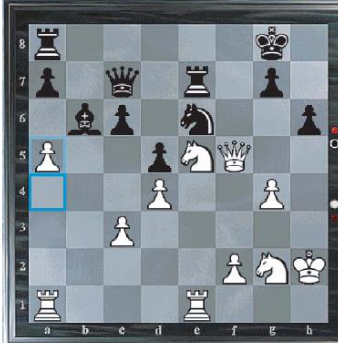
\includegraphics[width=36.96mm,height=94.45mm]{../../images/llm/page_029_img_01.png}%
\end{textblock*}

% deskripsi: Screenshot jendela email sebagai ilustrasi teknik Head-stega
% bbox normalisasi: [0.4620, 0.3140, 0.9450, 0.6520]
\begin{textblock*}{101.43mm}(97.02mm,93.26mm)
\noindent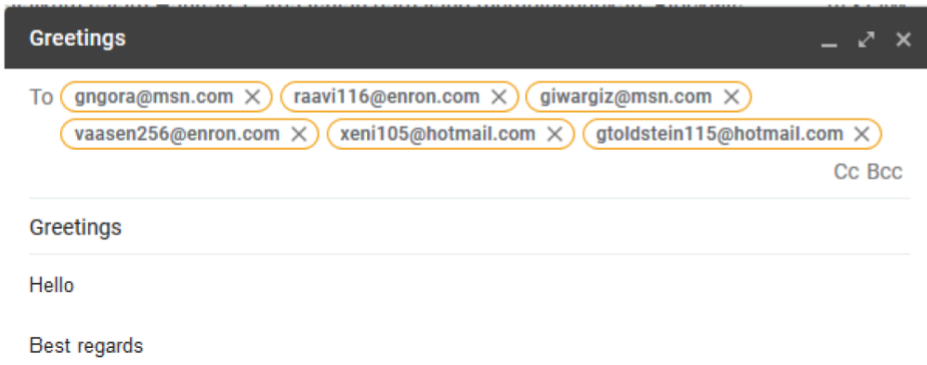
\includegraphics[width=101.43mm,height=100.39mm]{../../images/llm/page_029_img_02.png}%
\end{textblock*}

\end{document}
